\documentclass[11pt, oneside]{article}
\usepackage[margin=1in]{geometry}                % See geometry.pdf to learn the layout options. There are lots.
\geometry{letterpaper}                   % ... or a4paper or a5paper or ... 
%\geometry{landscape}                % Activate for for rotated page geometry
%\usepackage[parfill]{parskip}    % Activate to begin paragraphs with an empty line rather than an indent
\usepackage{graphicx}
\usepackage{amssymb}
\usepackage{amsmath}
\usepackage{array}
\usepackage{indentfirst}
\usepackage{mathptmx}
\usepackage{enumitem}
\usepackage{float}

\setcounter{secnumdepth}{3}

\title{APPM 4560 Laboratory 3 Report}
\author{Rhys Olsen\\
\texttt{rhys.olsen@colorado.edu}
 \and Jessica Petty\\
 \texttt{jessica.petty@colorado.edu}
 }
\date{November 16, 2016}

\begin{document}
\maketitle
\section{Simulating a Single Server Queue}
\subsection{Stationary Distribution of M/M/1-queue}
For an M/M/1 queue to have a stationary distribution, it is a necessary and sufficient condition that its arrival rate be less than its service rate. In the case of the queue provided, this means that $\lambda < \mu$.

\subsection{Distribution of a Stationary Queue}
When $X$ is stationary, this is equivalent to saying that it is in equilibrium. We know that an M/M/1-queue in equilibrium will have a geometric distribution of items inside. Now, given that $X_T$ is the number of items in the queue at time $T$, we can then say that the distribution of $X_T$, which is $P(X_T = t) = \pi(t)$, is geometric with success parameter $\frac{\lambda}{\mu}$.

\subsection{Busy Server}
When $X$ is stationary, the fraction of time that the server is \textit{not} busy is equivalent to the value $\pi(0)$. Conceptually, this is because the stationary distribution $\pi(x)$ represents the fraction of time that the queue has $x$ items in it. Clearly, if $x > 0$, this means the server is busy, as there are items in the queue, and when $x=0$ the server cannot be busy because there are no items in the queue, either waiting or being served.

For an M/M/1-queue, $\pi(0)=1-\frac{\lambda}{\mu}$. (PROOF can be found in notes if we decide it is necessary). Therefore, the fraction of time that the server \textit{is} busy is $1-\pi(0)=1-(1-\frac{\lambda}{\mu})=\frac{\lambda}{\mu}$

\subsection{Simulation of M/M/1-queue}
Now, to simulate an M/M/1-queue one can use the superposition argument of exponentials to create higher-rate event times, and then use thinning to deduce whether the observed event is an arrival or a departure. Using the following algorithm, one can also simulate an M/M/1-queue holding $n$ items over time $T$ with arrival rate $\lambda$ and service rate $\mu$.

\begin{enumerate}[leftmargin=30pt,labelindent=65pt,itemindent=30pt]
\item[\textsc{step 1:}] Set $i:=0$, $\tau:=0$, and $q(0):=(0,0)$
\item[\textsc{step 2:}] Simulate $U_1 \sim \text{Uniform}(0,1)$
\item[\textsc{step 3:}] If the queue is empty: set $i:=i-1$, $\tau:=q(i-1)(0) - \frac{\ln(U_1)}{\lambda}$, and $q(i):=(\tau, 1)$
\item[\textsc{step 4:}] Otherwise, if the queue is nonempty:
\begin{enumerate}[leftmargin=25pt,labelindent=65pt,itemindent=25pt]
\item[\textsc{step 4.1:}] Set $i:=i+1$ and set $\tau:=q(i-1)(0) - \frac{\ln(U_1)}{\lambda + \mu}$
\item[\textsc{step 4.2:}] Simulate $U_2\sim\text{Uniform}(0,1)$
\item[\textsc{step 4.3:}] If $U_2 \leq \frac{\lambda}{\lambda+\mu}$, set $q(i):=(\tau, 1)$ otherwise set $q(i):=(\tau,-1)$
\end{enumerate}
\item[\textsc{step 5:}] If $\tau > T$, return $q(:,i-1)$. Otherwise, go back to step 2.
\end{enumerate}

\subsection{Determining $X_T$}
Based on the provided pseudo-code, one can easily determine $X_T$. After running the given simulation, one will have a vector of tuples containing the time of the event and a value indicating whether the event was an arrival or a departure. To calculate $X_T$, starting with $n$ items in the queue, simply examine each element in the returned vector. If that item has a timestamp less than $T$ and if it is marked as an arrival, increment the count of items $n$ in the queue, otherwise if its time stamp is less than $T$ but it represents a departure, deprecate the count of items in the queue.

\subsection{Fraction of Busy Server Time}
To calculate the fraction of time that the server is busy between times $0 \text{ and } T$, again one will need to keep track of the number of items $n$ in the queue at any given time. This time, it will be necessary to create temporary variables in order to store all the values needed to compute the fraction of time the server is busy. Create and set variables $t:=0$, $s:=0$, and $e:=0$. Again, examine the vector containing the tuples of departures and arrivals. This time, if the item total reaches $0$ (or if the queue is instantiated with $0$ items), set the variable $s$ to be the time associated with the tuple being examined. Then, when the item total becomes non-zero, set the variable $e$ to be the time associated with the new tuple being examined. Then, set $t:=t+(e-s)$. Once the contents of the vector have been fully examined, the fraction of time that the server is busy is simply $\frac{T-t}{T}$.

\subsection{Determining Inter-Departure Times}
Again, once the simulation of an M/M/1-queue has been performed, determining the inter-departure times of items in the queue can be done by examining the contents of the returned vector. For each tuple in the vector, examine whether that tuple represents an arrival or a departure. If it represents a departure, store its departure time until the next departure is found. At that point, add the difference of these two times to another vector storing inter-departure times and repeat the process, storing the most recent departure time as the first departure time in the algorithm. In this way, upon reaching the end of the vector, all inter-departure times between time $0 \text{ and } T$ will have been calculated using the results of the simulation of an M/M/1-queue.

\subsection{Simulating $X_T$ when $X$ is Stationary}
Recall, when an M/M/1-queue is stationary, one expects is distribution to be Geometric with success parameter $\frac{\lambda}{\mu}$ where $\lambda$ is the rate of arrival to the queue and $\mu$ is the service rate of the queue. Therefore, simulating an M/M/1-queue with arrival rate $\lambda=1$ and service rate $\mu=2$ over time $T=50$, one would expect the number of items remaining in the queue at time $T$ to follow a geometric distribution with success parameter $1/2$. The findings of our simulation are consistent with this theory, as one can observe. After $10,000$ simulations of this M/M/1-queue, we found that in fact the number of items in the queue at time $T$ roughly followed a geometric distribution. The initial number of items in the queue $n$ is a random variable whose probability distribution is based on the stationary distribution of $X$.
\begin{figure}[H]
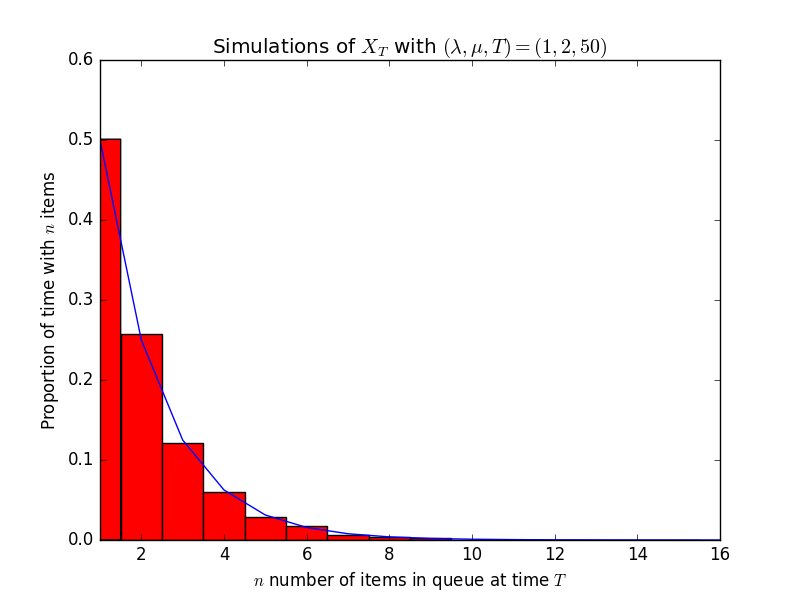
\includegraphics[scale=0.7]{simulation_xt}
\caption{The result of 10,000 simulations of $X_T$, an M/M/1-queue over time $T=50$ with arrival rate $\lambda=1$ and service rate $\mu=2$, against the expected probability mass function of a geometric distribution with success parameter 1/2.}
\label{fig:x}
\end{figure}

\subsection{Simulating Fraction of Time the Server is Busy}
After 10,000 simulations of an M/M/1-queue, the fraction of time that the server is busy stabilizes. Below is a plot of 10,000 simulations of an M/M/1-queue with arrival rate $\lambda$ and service rate $\mu$. These results are not surprising, as although one would expect the arrivals and departures would cause the server to be busy $\frac{\lambda}{\mu}=1/2$ of the time, the starting number of items in the queue is distributed based upon the stationary distribution, so often the server will begin needing to be busy rather than at rest, as would be the case if it started with no items every time.
\begin{figure}[H]
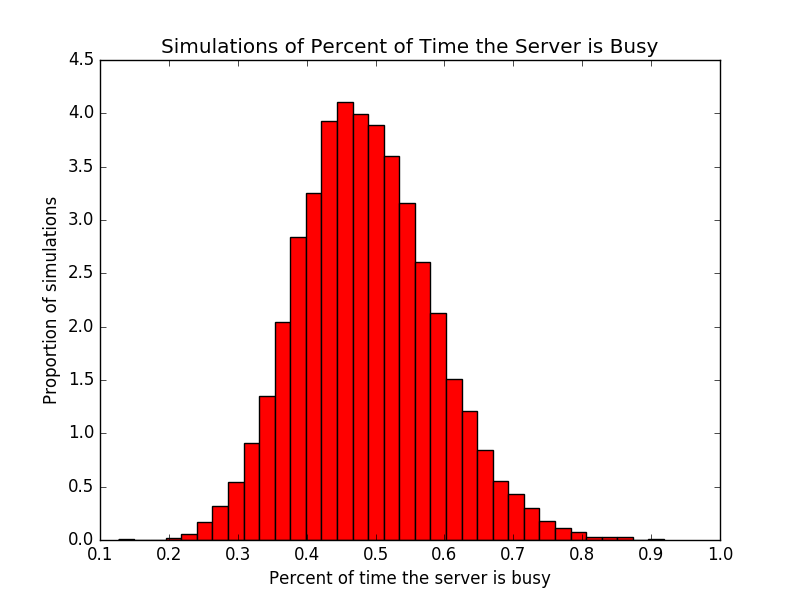
\includegraphics[scale=0.7]{busy_server}
\caption{10,000 simulations of an M/M/1-queue with arrival rate $\lambda=1$ and service rate $\mu=2$ for time $T=50$. The proportion of time the server is busy is unsurprising given the starting distribution of the number of items in the queue.}
\label{fig:x}
\end{figure}

\subsection{Demonstrating Output Process is HPP($\lambda$)}



\end{document}  
\grid
